\section{Trees}

\begin{definition}
    A \textbf{tree} is a graph that is connected and does not contain a cycle (a graph "contains a cycle" if it has a subgraph isomorphic to $C_n$ for some $n\geq3$).\\
    A \textbf{forest} is a graph that does not contain a cycle.\\
    A \textbf{leaf} is a vertex of a tree with degree $1$.
\end{definition}
\begin{example}
\hfill
    \begin{center}
        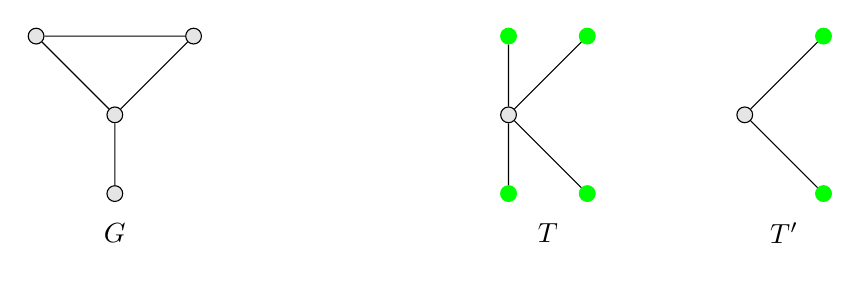
\begin{tikzpicture}[vertex/.style={circle, draw, fill=gray!20, minimum size=2mm, inner sep=0pt}]
        \node[vertex] (v1)  at (-6,2) {};
        \node[vertex] (v2)  at (-4,2)  {};
        \node[vertex] (v3)  at (-5,1)  {};
        \node[vertex] (v4)  at (-5,0)  {};
        \node at (-5,-0.5) {$G$};

        \draw (v4)--(v3)--(v1)--(v2)--(v3);

        \node[vertex, green] (v1') at (0,2) {};
        \node[vertex, green] (v2') at (1,2) {};
        \node[vertex] (v3') at (0,1) {};
        \node[vertex, green] (v4') at (1,0) {};
        \node[vertex, green] (v5') at (0,0) {};

        \draw (v1')--(v3')--(v2');
        \draw (v4')--(v3')--(v5');
        \node at (0.5,-0.5) {$T$};

        \node[vertex, green] (v1'') at (4,2) {};
        \node[vertex] (v3'') at (3,1) {};
        \node[vertex, green] (v5'') at (4,0) {};

        \draw (v1'')--(v3'')--(v5'');
        \node at (3.5,-0.5) {$T'$};
        \end{tikzpicture}
        \end{center}
    \begin{itemize}
        \item $G$ is not a tree nor a forest
        \item $T,T'$ are trees and forests
        \item $T\cup T'$ is a forest but not a tree
        \item All green vertices are leafs, all white vertices are not leafs
    \end{itemize}
    
\end{example}

\vspace{0.5cm}

\begin{lemma}
    Every tree $T$ with $n\geq 2$ vertices has one or two leafs.
\end{lemma}
\begin{proof}
    We iteratively construct a path $v_1,...,v_n$ as follows:\\
    Start with any edge $\{v_1,v_2\}\in E(T)$. Assume that we have constructed $v_1,...,v_k$. To construct $v_{k+1}$, we may assume that $v_k$ is not a leaf in $T$ (or we are done). Otherwise $v_k$ has a neighbour $v_{k+1}\neq v_{k-1}$. $v_{k+1}\neq v_i$ because $T$ is a tree and otherwise we would get a cycle ($v_i,...,v_k,v_{k+1}=v_k$). Add $v_{k+1}$ to the path and continue finite many steps (because there are only finitely many vertices). The algorithm just stated ends at a leaf.
\end{proof}
\begin{theorem}
    Let $G$ be a graph with $n$ vertices. The following are equal:
    \begin{enumerate}
        \item $G$ is a tree
        \item $G$ is connected with $n-1$ edges
        \item $G$ is connected and removing an edge disconnects it
        \item $G$ has exactly one path between each pair of distinct vertices
        \item $G$ has no cycle, but adding an edge creates a cycle
    \end{enumerate}
\end{theorem}
\begin{proof}
    "$1.\implies 2.$"\hfill \\
    Induction on $n$:\\
    $n=1$ is trivial\\
    Let $n\geq2$. By Lemma ($2.2$), $G$ has a leaf $v$. Removing $v$ and the unique edge incident to $v$ yields a tree $G'$. By induction $G'$ has $n-2$ edges so $G$ has $n-1$ edges.\par
    \vspace{0.3cm}
    "$2.\implies3.$"\\
    Suppose there is an edge $e\in E(G)$ and the resulting graph by removing $e$ is still connected. Keep removing as long as the resulting graph is still connected. Let $G'$ be the resulting graph. Observe that $G'$ is a spanning subgraph of $G$. $G'$ does not contain a cycle as otherwise we could remove one edge from the cycle. By "$1.\implies 2.$", applied to $G'$, we know that $G'$ has $n-1$ edges $\lightning$ because $G$ had $n-1$ edges and we removed at least one.\par
    \vspace{0.3cm}
    "$3.\implies 4.$"\\
    Suppose that there is a pair with $u,v\in V(G)$ s.t. there are two distinct paths $u_i,v_i$ between them. Let $i_0$ be the maximum index s.t. $u_i=v_i:\forall i\in\{1,...,i_0\}$. The edge $\{v_{i_0},v_{i_0+1}\}$ does not lie on the path $u_i$. The graph obtained by removing $\{v_{i_0},v_{i_0+1}\}$ is connected as for any walk using this edge we can use $u_i$ to go to $u$ to reach $v_{i_0}$ or $v$ to reach $v_{i_0+1}$.\par
    \vspace{0.3cm}
    "$4.\implies5.$\\
    If $G$ had a cycle, then there would exist two paths between each vertex on the cycle (clockwise + counter clockwise).\\
    Adding an edge creates a cycle: Let $u,v\in V(G)$ non adjacent. There is one path between the two. No adding an edge between $u,v$ creates a second path $\lightning$\par
    \vspace{0.3cm}
    "$5.\implies 1.$\\
    We only need to show that $G$ is connected. Suppose $u,v$ are not connected by a walk. Creating an edge between $u,v$ does not result in a cycle because for being isomorphic to $C_n$ one needs at least two walks between each of the vertices in the cycle but by assumption the only walk connecting $u,v$ is the newly added edge $\lightning$
\end{proof}
\vspace{1cm}
\begin{corollary}
    Every connected graph $G$ has a spanning tree.
\end{corollary}
\begin{proof}
\hfill \\
    Consider graphs on $n$ vertices, now do induction on the number of edges $m$. As $G$ is connected, $m\geq n-1$. If $m=n-1\implies G$ is a tree. If $m>n-1\implies G$ is not a tree. By ($2.3$) we can remove edges s.t. the resulting graph is connected. By induction it has a spanning tree, which is then also a spanning tree of $G$.
\end{proof}
\vspace{0.5cm}
\begin{theorem}[Matrix-tree theorem]
    Let $G$ be a graph with vertices $\{1,...n\}$, edges $\{e_1,...,e_m\}$. Let $Q=(q_{ij})$ with $q_{ij}=\begin{cases}
            -1 & \{i,j\}\in E \\
            0 & i\neq j:\{i,j\}\notin E\\
            \deg(i) & i=j
            \end{cases}$ 
    Let $Q_{ij}$ be the matrix obtained from $Q$ by removing the $i$-th row and the $j$-th column. Then the number of labelled spanning trees of G is $|\det(Q_{ij})|$, for any choice of $i,j$.
\end{theorem}
\vspace{0.5cm}
\begin{corollary}[Cayley's formula]
    The number of labelled spanning trees of $K_n$ is $n^{n-2}$ if $n\geq 2$.
\end{corollary}
\begin{proof}
    Define $Q$ as in $(2.5)$. \\
    $Q_{11}=\begin{pmatrix}
        n-1 & 1 & \cdots & 1\\
        1 & \ddots & & \vdots\\
        \vdots & & \ddots & 1\\
        1 &\cdots & 1 & n-1
    \end{pmatrix}\xrightarrow{}\bar Q_{11}=\begin{pmatrix}
        n-1 & -1 & -1&\cdots & -1\\
        -n & n &0&\cdots & 0\\
        -n & 0 & \ddots & & \vdots\\
        \vdots & \vdots & &\ddots &0\\
       -n &0&\cdots & 0 & n
    \end{pmatrix}\xrightarrow{}\hat Q_{11}=\begin{pmatrix}
        1 & \star & \cdots & \star\\
        0 & n & & \vdots\\
        \vdots & & \ddots & \star\\
        0 &\cdots & 0 & n
    \end{pmatrix}$\par
    $\implies |\det(Q_{11})|=|\det(\hat Q_{11})|=n^{n-1-1}=n^{n-2}$
\end{proof}